% !TeX root = Auswertung.tex
\subsection{Justieren des Lasers}
\begin{figure}[h!]
\centering
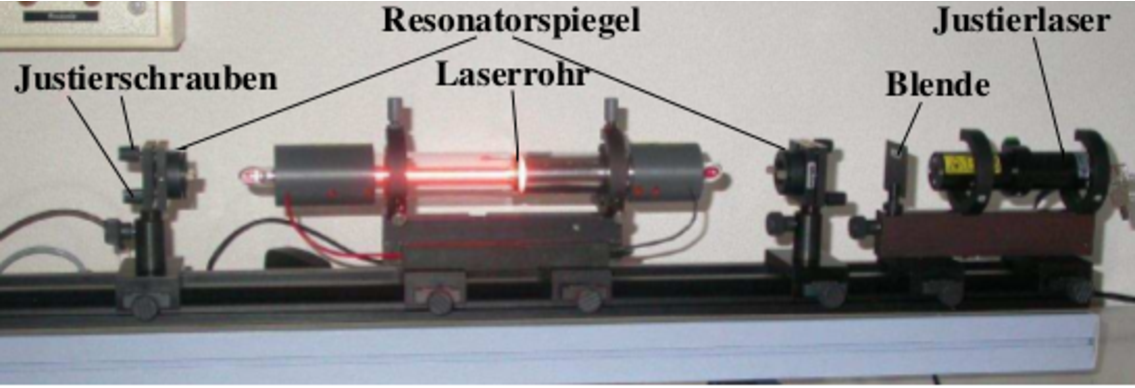
\includegraphics[scale=0.75]{../Grafiken/Aufbau.pdf}
\caption{Der Aufbau des HeNe-Lasers\cite{V61}}\label{Aufbau}
\end{figure}
Für den Grundaufbau stehen verschiedene Komponenten zur Verfügung, eine optische Schiene an deren einen Ende ein Justierlaser befestigt ist, verschiedene Spiegel sowie Halterungen für diese und zwei Blenden mit Fadenkreuz und Halterungen.\\ 
Als erstes wird eine Blende je vor dem Justierlaser, sowie ans andere Ende der Schiene befestigt. Mithilfe der Justiershrauben am Laser wird er so ausgerichtet, dass die Beugungsringe des Justierlasers in der Mitte des Fadenkreuz der hinteren Blende sind.\\
Als nächstes wird der teil durchlässige Spiegel mit der Reflektierenden Seite zum Justierlaser gerichtet auf die schiene gestellt. Der Spiegel wird, mithilfe der Justierschrauben vom Spiegel, so eingestellt das der helle Rückreflex in der Mitte der Blende ist, die vor dem Laser steht.\\ 
Nun wird der zweite Spiegel auf der schiene zwischen dem Ersten Spiegel und der Blende, vor dem Justielaser befestigt, und mit der Reflektierenden Seite zum ersten Spiegel gewannt. Dieser Spiegel wird eingestellt wie der erste Spiegel, mit dem unterschied das der diffuse Rückreflex in die Mitte des Fadenkreuz sein muss. 

\begin{table}
\centering
\begin{tabular}{c c c}
Spiegel & Bezeichnung & Oberflächenbeschaffenheit \\\hline
plan & flat/flat & $HR$ (Hohe Reflexivität) $R\ge 99\%$\\
konkav & $r=1000mm$/flat & $HR$ (Hohe Reflexivität) $R\ge 99\%$\\
konkav & $r=1400mm$/flat & $HR$ (Hohe Reflexivität) $R\ge 99\%$\\
konkav & $r=1400mm$/flat & $OC$ (Auskopplung) $T=1.5,...1.8\% $
\end{tabular}
\caption{Die Daten der zur Verfügung Stehenden Spiegeln.\cite{V61}}\label{Eigenschaften}
\end{table}
